\documentclass{standalone}

 \usepackage{tikz}

 \begin{document}

 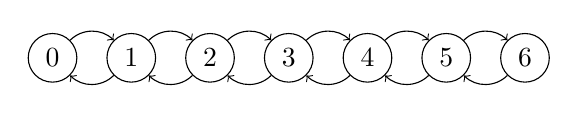
\begin{tikzpicture}

     \node (A) at (0, 0) [draw, circle] {0};
     \node (B) at (1, 0) [draw, circle] {1};
     \node (C) at (2, 0) [draw, circle] {2};
     \node (D) at (3, 0) [draw, circle] {3};
     \node (E) at (4, 0) [draw, circle] {4};
     \node (F) at (5, 0) [draw, circle] {5};
     \node (G) at (6, 0) [draw, circle] {6};

     \draw [->] (A) to [out=45, in=135] (B);
     \draw [->] (B) to [out=45, in=135] (C);
     \draw [->] (C) to [out=45, in=135] (D);
     \draw [->] (D) to [out=45, in=135] (E);
     \draw [->] (E) to [out=45, in=135] (F);
     \draw [->] (F) to [out=45, in=135] (G);

     \draw [->] (B) to [out=-135, in=-45] (A);
     \draw [->] (C) to [out=-135, in=-45] (B);
     \draw [->] (D) to [out=-135, in=-45] (C);
     \draw [->] (E) to [out=-135, in=-45] (D);
     \draw [->] (F) to [out=-135, in=-45] (E);
     \draw [->] (G) to [out=-135, in=-45] (F);


 \end{tikzpicture}

 \end{document}
